\chapter[The ReReReRe Detector]{ReReReRe: A Permutation-Based Coherence Detector}
\label{ch:rerere}

\section{Motivation and Core Idea}

Chapter~1 closed on a gap. The detection methods in widest use are strongest on
\emph{consistent} careless responding---straightlining, acquiescence, machine-like
regularity---and weakest on \emph{inconsistent} careless responding, where a
respondent's answers vary across items but bear no coherent relationship to item
content. Random and mixed responding are the hardest patterns to prevent and the
most damaging to covariance-based analyses, yet the only established index that
targets them directly, the psychometric-synonym statistic
\parencite{meade2012identifying}, operates on a handful of hand-selected item
pairs. This chapter introduces \emph{ReReReRe}, a detector built specifically to
exploit the full correlational structure of a multi-construct questionnaire in
order to identify inconsistent careless responding.

The core idea is a single observation made operational. An attentive
respondent's answer to one item is informative about their answer to a
correlated item, because both items load on a shared latent factor
(Section~\ref{sec:efa}). A careless respondent's answers to the same pair are
\emph{incoherent}: the cross-item structure that the sample as a whole exhibits
is absent in their individual profile. ReReReRe measures, for each respondent,
how much of the sample's pairwise structure their own answers reproduce, and
compares that quantity against a baseline obtained by permutation. The result is
a per-respondent z-score: high when the respondent is more coherent than chance
(attentive), low or negative when they are no more coherent than randomly paired
items would predict (potentially careless). Because the baseline is built
separately for each respondent, the method is \emph{self-calibrating}: it makes
no distributional assumption about the coherence statistic, sidestepping the
normality problems that, as Chapter~1 noted, cripple the chi-square cutoff for
Mahalanobis distance on Likert data.

\section{The Algorithm}

\subsection{Individual-level coherence}

Let $X$ be the $N \times J$ matrix of responses ($N$ respondents, $J$ items).
The sample-level correlation matrix $R$ summarizes how items relate across
respondents. ReReReRe selects a set of $k$ item pairs $\{(a_1,b_1),\dots,
(a_k,b_k)\}$ that the sample deems related (Section~3.2.2), and then, for each
respondent $r$, forms the two vectors of that respondent's answers to the
left-hand and right-hand members of the pairs,
\[
\mathbf{u}_r = \big(X_{r,a_1}, X_{r,a_2}, \dots, X_{r,a_k}\big), \qquad
\mathbf{v}_r = \big(X_{r,b_1}, X_{r,b_2}, \dots, X_{r,b_k}\big).
\]
The respondent's \emph{coherence} is a weighted association between
$\mathbf{u}_r$ and $\mathbf{v}_r$, with each pair contributing in proportion to
its sample-level $|r|$,
\begin{equation}
C_{\text{obs}}(r) \;=\; \sum_{j=1}^{k} w_j \, \tilde{u}_{r,j}\,\tilde{v}_{r,j},
\qquad w_j = \frac{|R_{a_j b_j}|}{\sum_{l} |R_{a_l b_l}|},
\label{eq:coherence}
\end{equation}
where $\tilde{u}, \tilde{v}$ denote the item-standardized values. Strong pairs
count more than weak ones, but no pair is discarded outright. The crucial point
is that Equation~\ref{eq:coherence} is computed \emph{down a respondent's row},
not across respondents: it asks whether \emph{this person} answered the coupled
pairs coherently.

\subsection{Pair selection: two regimes}

How the $k$ pairs are chosen depends on questionnaire length, because the signal
ReReReRe relies on comes from the total number of high-correlation pairs
available, and that number scales very differently for short and long
instruments. ReReReRe therefore switches automatically between two regimes at a
threshold of 60 items (the \texttt{mode = "auto"} default).

\textbf{Weighted regime} (used for $J \le 60$ items). Every one of the
$\binom{J}{2}$ item pairs is included, each weighted by its absolute sample
correlation as in Equation~\ref{eq:coherence}. With short questionnaires there
are too few strongly correlated pairs to select a clean subset, so discarding
any of them throws away signal; using all pairs but down-weighting the weak ones
extracts the most from limited structure.

\textbf{Coupled regime} (used for $J > 60$ items). Only the top
\texttt{corProp} fraction of pairs by absolute correlation is retained (default
3\%), subject to a floor of \texttt{min\_pairs} = 15. With long questionnaires
the strongest pairs carry a clean, redundant signal, and restricting attention
to them sharpens the contrast between attentive and careless respondents while
keeping the computation tractable.

The switch is automatic and recorded in the output (\texttt{mode\_used}); a user
can override it to force either regime. Calibration studies confirm a crossover
near 60 items: below it the weighted regime wins by up to $0.06$ MCC, above it
the coupled regime wins by a similar margin.

\subsection{The permutation baseline and the z-score}

A high coherence is only meaningful relative to what coherence the same
respondent would show over pairs with \emph{no} shared structure. ReReReRe
constructs this baseline by permutation (Section~\ref{sec:perm}). For each of
\texttt{iterations} = 100 rounds, it draws $k$ \emph{random} item pairs from the
matrix, recomputes the same weighted coherence as in
Equation~\ref{eq:coherence}, and thereby obtains, for each respondent, a null
distribution $\{C_{\text{rand}}(r,1), \dots, C_{\text{rand}}(r,100)\}$. The
respondent's score is the standardized distance of their observed coherence from
this personal baseline,
\begin{equation}
z_{\text{RR}}(r) \;=\;
\frac{C_{\text{obs}}(r) - \operatorname{mean}_s C_{\text{rand}}(r,s)}
{\operatorname{sd}_s C_{\text{rand}}(r,s)} .
\label{eq:zrr}
\end{equation}
This is the permutation z-score of Equation~\ref{eq:z}, specialized to coherence.
A respondent is flagged as careless when $z_{\text{RR}}$ falls below a
threshold (Section~3.5). The algorithm is summarized in the box below.

\begin{quote}
\small
\textbf{Algorithm: ReReReRe (standard mode).}
\begin{enumerate}\setlength{\itemsep}{1pt}
\item Rescale each item (default: divide by its observed maximum;
      Section~3.4).
\item Compute the sample correlation matrix $R$; record the sign of each
      correlation.
\item \emph{Sign alignment}: for each pair with $R_{ab} < 0$, reverse-code
      column $b$ (Section~3.3).
\item Select pairs: all pairs (weighted, $J\le 60$) or the top-$k\%$ by $|r|$
      (coupled, $J>60$).
\item Compute each respondent's weighted coherence $C_{\text{obs}}$
      (Eq.~\ref{eq:coherence}).
\item Repeat 100 times: draw $k$ random pairs, sign-align, compute
      $C_{\text{rand}}$.
\item Convert to a per-respondent z-score $z_{\text{RR}}$ (Eq.~\ref{eq:zrr}).
\item Flag respondents with $z_{\text{RR}} \le$ threshold (default $1.5$, or
      auto-calibrated).
\end{enumerate}
\end{quote}

In R the entire procedure is a single call,
\texttt{ReReReRe(data)}, returning a data frame with each respondent's
$z_{\text{RR}}$, the flag, and metadata (the regime used, the calibrated
threshold, the estimated number of factors). The default parameters are listed
in Table~\ref{tab:params}.

\begin{table}[t]
\centering
\caption{Default parameters of \texttt{ReReReRe()} and their role.}
\label{tab:params}
\small
\begin{tabular}{L{0.22\linewidth} L{0.16\linewidth} L{0.50\linewidth}}
\toprule
\textbf{Parameter} & \textbf{Default} & \textbf{Role} \\
\midrule
\texttt{mode} & \texttt{"auto"} & Weighted if $J\le 60$, coupled if $J>60$ \\
\texttt{corProp} & $0.03$ & Fraction of top-$|r|$ pairs kept (coupled regime) \\
\texttt{min\_pairs} & $15$ & Floor on the number of coupled pairs \\
\texttt{iterations} & $100$ & Number of permutation rounds for the baseline \\
\texttt{align\_signs} & \texttt{TRUE} & Reverse-code negatively-correlated pairs \\
\texttt{rescale} & \texttt{"proportion"} & Per-item rescaling for mixed scales \\
\texttt{z\_threshold} & $1.5$ & Flagging cutoff (or \texttt{auto}) \\
\texttt{auto\_z} & \texttt{FALSE} & Calibrate the cutoff from total item count \\
\bottomrule
\end{tabular}
\end{table}

\section{Reverse-Coded Items: Sign Alignment}

Questionnaires routinely include \emph{reverse-keyed} items, worded so that
agreement indicates \emph{less} of the trait. Such an item correlates
\emph{negatively} with same-trait items keyed in the usual direction. This
creates a subtle but fatal problem for any method that aggregates correlations
across pairs. If the coherence of Equation~\ref{eq:coherence} mixes
positively-keyed pairs (which contribute positive products for an attentive
respondent) with negatively-keyed pairs (which contribute negative products),
the two cancel inside the sum, and even a perfectly coherent respondent receives
$C_{\text{obs}} \approx 0$. Every respondent then looks equally incoherent, and
the z-score carries no signal.

The defect is not hypothetical. It was discovered on the Robie HEXACO-60 data,
where 52\% of the coupled pairs were oppositely keyed: with the pairs left
unaligned, every respondent received $z_{\text{RR}} \approx 0$ (mean observed
coherence $0.078$ versus a baseline mean of $0.084$), and the detector's area
under the curve sat at chance. The fix, controlled by \texttt{align\_signs}
(default \texttt{TRUE}), is to use the \emph{sign} of each pair's sample-level
correlation to align the pair before computing coherence: wherever
$R_{ab} < 0$, column $b$ is reverse-coded (mapped by
$x \mapsto (\max_b + \min_b) - x$) so that the pair contributes positively for a
coherent respondent. The same alignment is applied to the random pairs of the
permutation baseline, so the null distribution is comparable. With the fix in
place on the Robie data, mean coherence rose to $0.299$, the mean z-score to
$3.49$, and the area under the curve from $0.47$ to $0.66$.

Sign alignment is more than data hygiene: it is what lets ReReReRe operate on
real questionnaires \emph{without} requiring the user to recode reverse-keyed
items by hand. The procedure is transparent and emits a warning only when it is
disabled in the presence of negatively-keyed pairs.

\section{Mixed Response Scales: Rescaling}

A second real-data complication is \emph{heterogeneous response scales}: a
battery that mixes, say, 1--4 and 1--7 items. Because the Pearson correlation in
Equation~\ref{eq:coherence} is sensitive to the numerical spacing of the
response options, longer-range items would otherwise dominate a respondent's
coherence simply by virtue of their larger spread. ReReReRe addresses this with
an optional per-item rescaling step (\texttt{rescale}), applied before any
correlation is computed.

The default, \texttt{"proportion"}, divides each item by its observed maximum.
This choice is principled. Section~\ref{sec:corr} noted that the Pearson correlation is
invariant to identical affine transforms applied to all items: on a
\emph{homogeneous}-scale questionnaire every column is divided by the same
constant, so the coherence is provably unchanged---the rescaling costs nothing.
On a \emph{heterogeneous}-scale questionnaire it equalizes the contribution of
items measured on different ranges. On a stress test of 80 items split between
1--4 and 1--7 scales, proportion rescaling lifted MCC from $0.32$ (no rescaling)
to $0.43$, while leaving uniform-scale results numerically identical. More
aggressive options are exposed for advanced users---\texttt{"minmax"} and
\texttt{"zscore"}---and \texttt{"none"} reproduces the legacy behaviour while
warning when item ranges are heterogeneous. The recommendation is nonetheless to
keep response scales uniform where possible; rescaling is a safeguard, not a
substitute for clean design.

\section{Threshold Selection and Auto-Calibration}

The z-score of Equation~\ref{eq:zrr} is continuous; flagging requires a cutoff.
Two findings make this less fraught than it sounds. First, the method is
\emph{not} sharply threshold-sensitive: across a wide range of conditions, any
cutoff between roughly $1.0$ and $2.0$ performs near-optimally, with a flat
plateau of detection quality. The recommended universal default is
$z_{\text{threshold}} = 1.5$, interpreted as ``the respondent's coherence is
$1.5$ standard deviations above their own random baseline.''

Second, where one wants to do better than a universal default, the optimal cutoff
has a clean and interpretable dependence on questionnaire size. Figure~\ref{fig:ushape}
shows the optimal threshold as a function of the number of factors, holding
items per factor fixed. The curve is \emph{U-shaped}: at very low factor counts
the z-scores of attentive and careless respondents overlap heavily, forcing a
low threshold to catch anyone; as the number of factors grows the two
distributions separate, and a \emph{higher} threshold becomes optimal because it
buys specificity without sacrificing sensitivity. The blue point cloud also
encodes detection quality through marker size, which grows visibly from left
(small, $\text{MCC} < 0.15$) to right (large, $\text{MCC} > 0.5$): more factors
mean both a higher optimal threshold and better detection.

\begin{figure}[t]
\centering
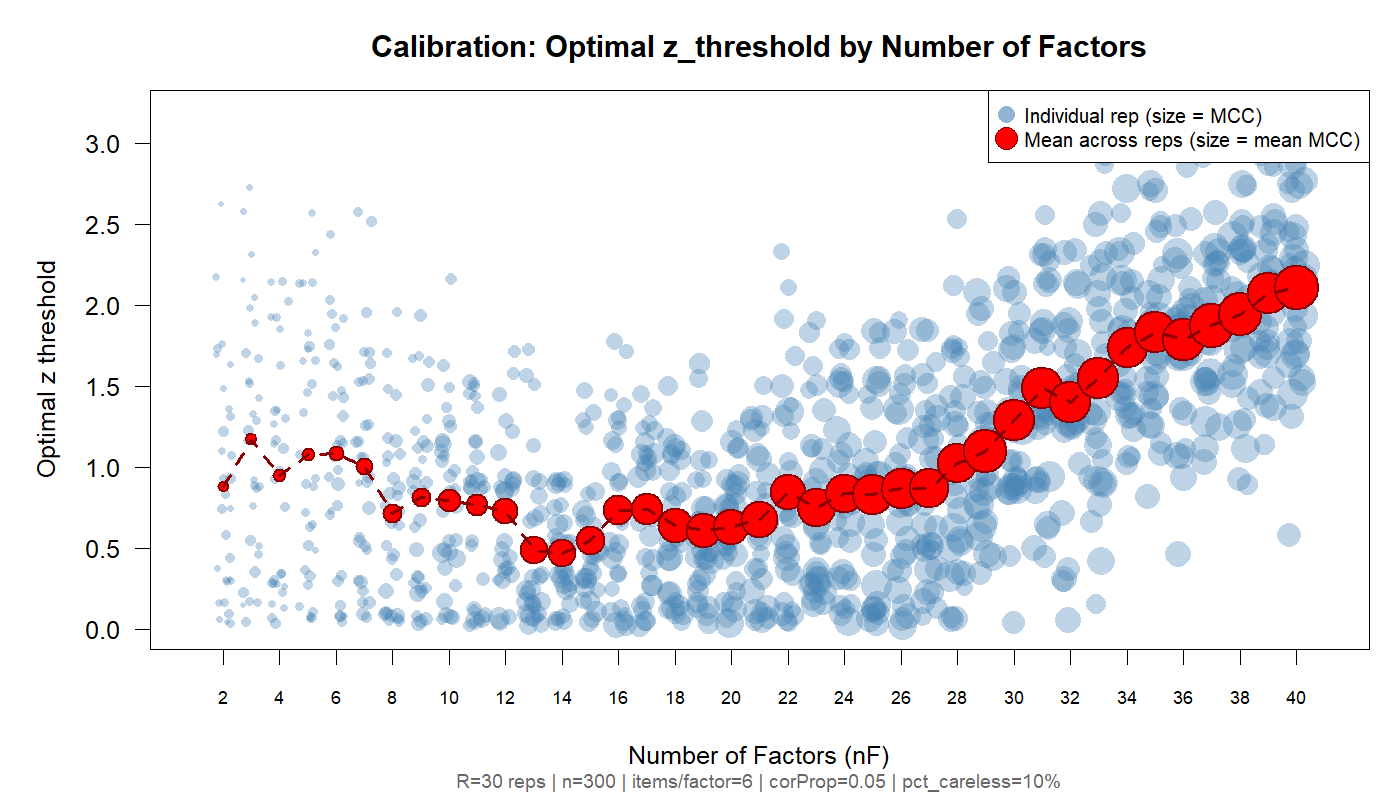
\includegraphics[width=0.92\linewidth]{figures/fig_calibration_ushape.png}
\caption{Optimal z-threshold as a function of the number of factors (items per
factor fixed at 6, $n = 300$, 10\% careless, 30 replications). Blue points are
individual replications (size $\propto$ MCC); red points are replication means.
The optimal threshold follows a U-shape, reaching a minimum near $z \approx 0.5$
at 13--15 factors and rising to $z \approx 2.1$ at 40 factors.}
\label{fig:ushape}
\end{figure}

Rather than calibrate on the number of factors alone, the implementation uses
the better predictor identified by a two-dimensional calibration study: the
\emph{total} number of items. A simple linear rule,
$z \approx 0.505 + 0.0042 \times (\text{total items})$, explains roughly twice
the variance of a rule based on the factor count, because what governs the
separation of the z-score distributions is the total number of high-correlation
pairs available, which scales with both the number of factors and the items per
factor. Setting \texttt{auto\_z = TRUE} activates this calibration:
ReReReRe estimates the number of factors by parallel analysis (Section~\ref{sec:efa}),
looks up the calibrated threshold, and applies it. In aggregate, auto-calibration
performs about as well as the fixed $z = 1.5$ default, confirming that the method
does not demand careful tuning; its value is convenience, removing a parameter
choice for non-technical users.

\section{Intrinsic Properties}

Before comparing ReReReRe to other detectors, it is worth characterizing how its
performance depends on questionnaire structure, because those dependencies
explain both its strengths and its limits. The picture below comes from a large
simulation multiverse crossing the number of factors, items per factor, sample
size, and careless base rate, with the structure of each dataset known by
construction.

\subsection{Signal grows with dimensionality}

The mechanism behind ReReReRe predicts that more factors should yield a cleaner
separation between attentive and careless respondents, because a richer factor
structure offers more coherent pairs against which incoherence stands out.
Figure~\ref{fig:zsep} confirms this directly. It plots the mean z-score of
attentive and of careless respondents as the number of factors increases. At
four factors the two groups overlap almost completely (a gap of about $0.48$);
by thirty factors they are separated by nearly three standard deviations (a gap
of about $2.81$). The attentive curve climbs steeply while the careless curve
stays low, and the $z = 1.5$ default sits cleanly between them across most of the
range.

\begin{figure}[t]
\centering
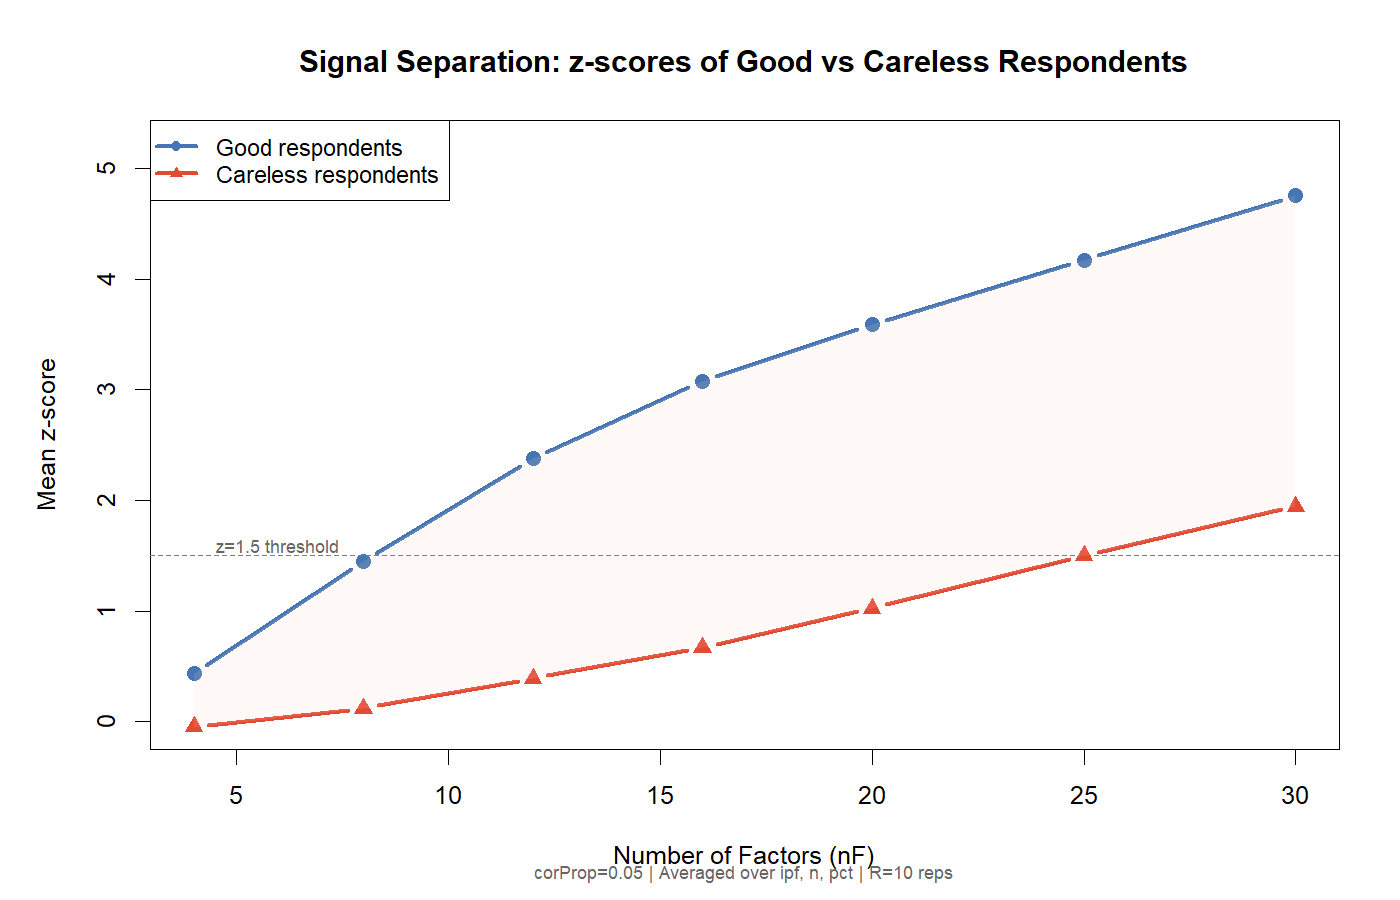
\includegraphics[width=0.92\linewidth]{figures/fig_z_separation.png}
\caption{Mean z-score of attentive (``good'') versus careless respondents as a
function of the number of factors (averaged over items per factor, sample size,
and base rate; 10 replications). The separation grows quasi-linearly with
dimensionality, explaining the method's scaling advantage. The dashed line marks
the $z = 1.5$ default cutoff.}
\label{fig:zsep}
\end{figure}

\subsection{Total length is the unifying predictor}

Decomposing the variance in detection quality, the two strongest drivers are the
items per factor ($\eta^2 = 0.31$) and the number of factors ($\eta^2 = 0.26$);
sample size and base rate matter much less. Crucially, neither factor count nor
items per factor alone is the right summary---their \emph{product}, the total
questionnaire length, is. Figure~\ref{fig:totalitems} plots detection quality
against total items and collapses the separate effects onto a single saturating
curve: MCC rises steeply up to roughly 150 items and then plateaus, with a slight
decline beyond about 250 items where the number of items begins to approach the
number of respondents and individual-level correlations grow noisy. The
practical reading is that ReReReRe should be described in terms of
\emph{total length}, not number of constructs: a 120-item questionnaire of 12
factors with 10 items each detects far better than a 75-item questionnaire of 25
factors with 3 items each, despite the latter's higher factor count.

\begin{figure}[t]
\centering
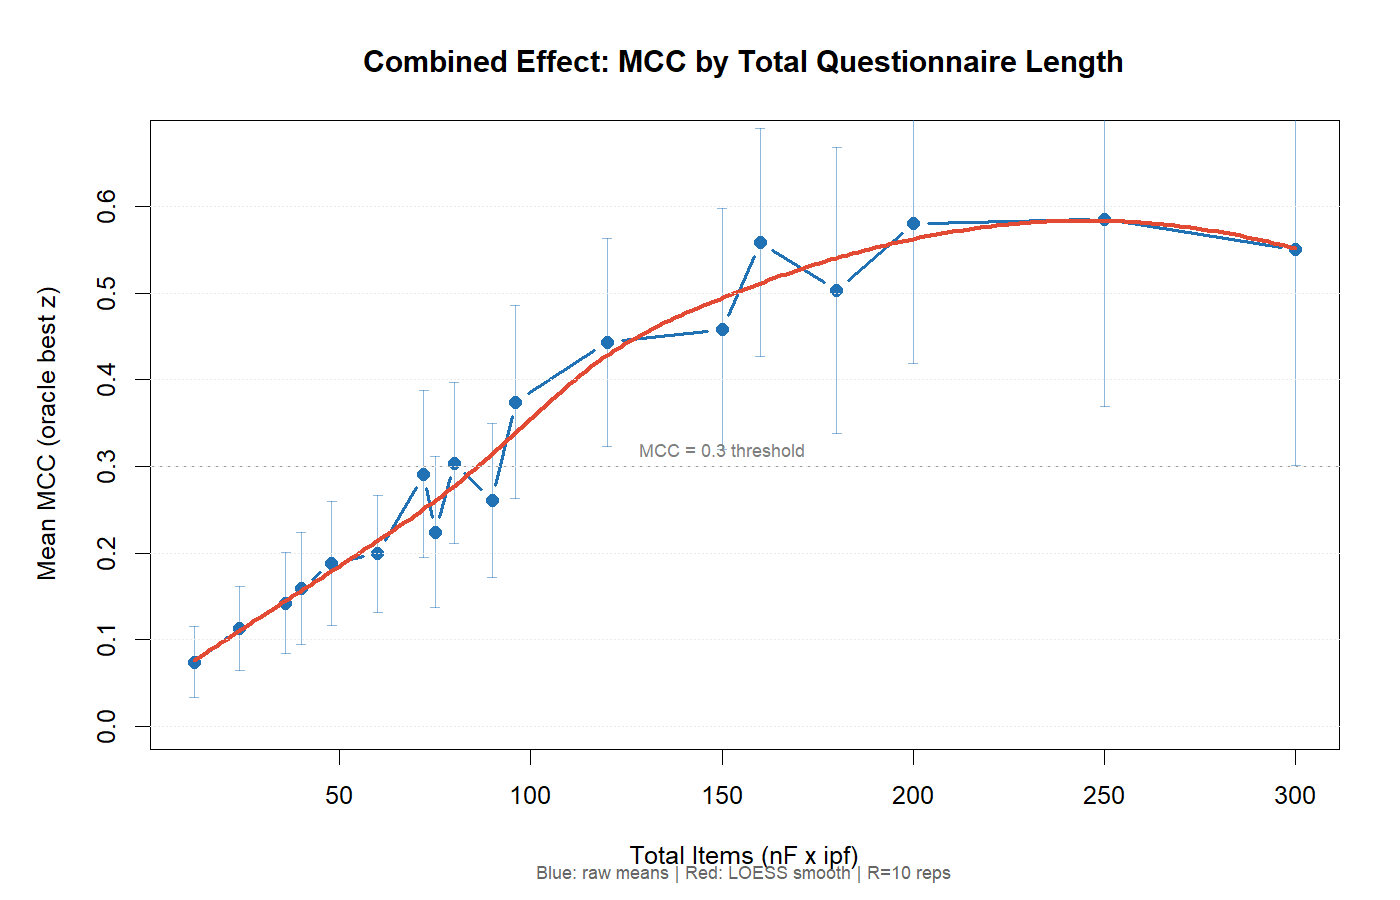
\includegraphics[width=0.92\linewidth]{figures/fig_mcc_total_items.png}
\caption{Detection quality (oracle-best MCC) as a function of total
questionnaire length (number of factors $\times$ items per factor). Blue points
are condition means with $\pm 1$ SD bars; the red curve is a LOESS smooth. MCC
saturates above roughly 150 items.}
\label{fig:totalitems}
\end{figure}

\subsection{Detection by careless pattern}

Broken down by the type of injected careless responding, ReReReRe detects all
three inconsistent patterns at comparable rates: longstring at about 83\%, mixed
at about 81\%, and random at about 79\% (averaged over the favorable threshold
range). This even profile is expected, since all three corrupt the cross-pair
structure the method monitors. The limits of the method, examined next, lie not
in any one inconsistent pattern but in the \emph{consistent} patterns it is not
designed to see.

\section{Benchmark Comparison: ReReReRe versus Mahalanobis}

Mahalanobis distance is the most widely used multivariate-outlier index for
careless detection (Section~1.4.2), and it is the natural benchmark for
ReReReRe. The comparison below was run on \emph{identical} simulated datasets, so
the two detectors face exactly the same data. Two framings are necessary,
because the comparison hinges on how each method's threshold is set.

\subsection{Practical thresholds: the decisive contrast}

In practice, Mahalanobis distance is applied with a fixed cutoff: respondents
whose squared distance exceeds the chi-square critical value at $\alpha = .001$,
with degrees of freedom equal to the number of items, are flagged
\parencite{meade2012identifying, curran2016methods}. This is the Mahalanobis
counterpart of ReReReRe's $z = 1.5$ default---a rule requiring no access to
labels. Under this realistic, label-free comparison the two methods are not
close. The chi-square rule is \emph{essentially non-functional} on Likert data:
its sensitivity is between $0.4\%$ and $1.9\%$, so it catches almost no careless
respondents, for an MCC of about $0.06$. ReReReRe with its fixed default reaches
an MCC of about $0.27$ over the same conditions---more than four times higher.
The reason is exactly the one developed in Chapter~1: the chi-square reference
distribution assumes multivariate normality, which Likert data violate badly, so
the nominal cutoff is far too conservative. ReReReRe's permutation baseline makes
no such assumption.

\subsection{Oracle thresholds and the threshold-free view}

It might be objected that Mahalanobis distance could do better with a tuned
cutoff. This is true, but the tuning requires the true labels---an
\emph{oracle} no analyst possesses. Even granting Mahalanobis its oracle-best
threshold per condition, ReReReRe (also at its oracle best) overtakes it as
dimensionality grows: the two are tied near ten factors (MCC $\approx 0.37$ for
both), after which ReReReRe pulls ahead, reaching MCC $\approx 0.57$ at
twenty-five factors versus $\approx 0.39$ for Mahalanobis, whose performance
stays roughly flat. The fairest single comparison is the threshold-free area
under the curve, which removes the thresholding question entirely
(Section~\ref{sec:metrics}). Here ReReReRe's AUC, computed with fully fixed defaults, climbs
from $0.59$ at four factors to $0.84$ at twenty-five, overtaking Mahalanobis
(flat at about $0.64$) from eight factors upward. The conclusion is consistent
across framings: Mahalanobis is a slightly better detector for very short
questionnaires but does not scale, whereas ReReReRe scales strongly with
questionnaire length and, under any realistic thresholding, dominates by a wide
margin.

The two methods detect different things, and this is the deeper point.
Mahalanobis distance flags multivariate \emph{outliers}---respondents far from
the sample centroid---whether careless or merely unusual. ReReReRe flags
\emph{incoherence}---a breakdown of the cross-factor structure. The next
chapter exploits this complementarity rather than choosing between the two.

\section{Design Alternatives Explored}

The canonical \texttt{ReReReRe()} described above---the weighted/coupled
auto-switch with sign alignment and proportion rescaling---was selected after a
broad search over alternative formulations. They are noted here briefly for
completeness; none displaced the canonical method as the recommended detector.

\emph{Factor-guided pair selection} (an EFA-based variant, exposed as
\texttt{ReReReRe\_F()}) chooses within-factor pairs from an exploratory factor
solution rather than by raw correlation. It wins on \emph{simulated} data, where
the factor structure is clean, but loses on \emph{real} validation datasets,
where parallel analysis on noisy, cross-loaded data produces poor factor
assignments; the empirical top-$|r|$ ranking of the coupled regime proved more
robust to contamination. \emph{Iterative} re-estimation (re-running the factor
solution on the respondents judged attentive, then re-scoring) gave a small
improvement on mid-length questionnaires but not elsewhere. A \emph{split-half}
scorer and a \emph{variance penalty} (which pushes near-zero-variance
straightliners toward negative z) each helped on specific partial-corruption or
consistent-careless cases but did not improve overall classification enough to
justify added complexity. The lesson from these experiments---that a method's
edge on simulated data need not survive on real data---shaped the validation
philosophy of the chapters that follow. The variant code remains in the software
for reference but is not part of the recommended pipeline.

\section{Limitations and the Case for an Ensemble}

ReReReRe is a strong standalone detector of inconsistent careless responding,
but it has three limits, and naming them sets up the next chapter. First, it is
\emph{weak at low dimensionality}: with few factors the z-score distributions of
attentive and careless respondents overlap (Figure~\ref{fig:zsep}), and
detection is modest below roughly eight factors. Second, by construction it
targets \emph{inconsistent} careless responding and adds little on
\emph{consistent} patterns---pure straightlining and acquiescence---which a
simple longstring or low-variability rule already catches perfectly. Third, even
at its best a single threshold leaves a gap to the oracle, because no
label-free rule can perfectly separate the two classes.

Each limit is the mirror image of a strength of some other detector. Mahalanobis
distance and longstring catch the consistent patterns ReReReRe misses;
low-variability indices catch straightlining outright. This complementarity
suggests that the right way to use ReReReRe is not alone but as one informative
feature among several, combined by a classifier that learns when to trust each.
That is the subject of Chapter~4, which embeds ReReReRe in a Random Forest
ensemble alongside the auxiliary detectors and quantifies, with the confidence
intervals introduced in Section~\ref{sec:boot}, exactly how much the coherence signal
contributes.

